\begin{mainquestion}{inductorwaveforms}{Messing with Inductors}

\questionpoints
Assume the switch below has been closed for an infinitely long time. At time $t = 0$ the switch is opened.

\begin{center}
\begin{circuitikz}
  \draw
    (0,3) to[V,l_=$\SI{3}{\volt}$,i=$i$] (0,0)
    (0,3) -- (1,3) to[R,l=$\SI{30}{\ohm}$] (3,3)
    to[L,l=$\SI{10}{\milli\henry}$,-*] (5,3)
    to[R,l=$\SI{2}{\kilo\ohm}$] (5,0)
    (5,3) -- (7,3) to[ospst=$S_1$,-] (7,0) -- (0,0);
  \draw
    (7,3) to[short,*-] (8,3)
    to[open, v^>=$v_\mathrm{out}$,o-o] (8,0)
    to[short,-*] (7,0);
\end{circuitikz}
\end{center}

% =========================================================
\begin{partquestion}{maxvoltage}
{What is the maximum voltage that occurs across $V_\mathrm{out}$?}

\begin{answer}[1in]
When the switch is closed the current flowing through the inductor is $\SI{0.1}{\ampere}$.
The instant after the switch is opened, the inductor keeps the same amount of current flowing, $\SI{0.1}{\ampere}$. At that instant, the $\SI{0.1}{\ampere}$ of current flows into the $\SI{2}{\kilo\ohm}$ resistor and develops a voltage of
\[
V_\mathrm{out} = (0.1)(2000) = \boxed{200\text{ V}}.
\]
\end{answer}

\end{partquestion}

Suppose you would like to limit the output voltage from going too high using a diode, like below.
    
    \begin{center}
    \begin{circuitikz}
      \draw
        (5,3) -- (5,5) to[D,l=$D$,i=$i_D$, v=$V_F$] (0,5) to[short,-*] (0,3);
    
      \draw
        (0,3) to[V,l_=$\SI{3}{\volt}$,i=$i$] (0,0)
        (0,3) -- (1,3) to[R,l=$\SI{30}{\ohm}$] (3,3)
        to[L,l=$\SI{10}{\milli\henry}$,-*] (5,3)
        to[R,l=$\SI{2}{\kilo\ohm}$] (5,0)
        (5,3) -- (7,3) to[ospst=$S_1$,-] (7,0) -- (0,0);
    
      \draw
        (7,3) to[short,*-] (8,3)
        to[open, v^>=$v_\mathrm{out}$,o-o] (8,0)
        to[short,-*] (7,0);
    \end{circuitikz}
    \end{center}

% =========================================================
\begin{partquestion}{diodevoltage}
{Suppose the diode has a forward voltage of $V_F=\SI{0.7}{\volt}$. What is the maximum voltage at the output $V_\mathrm{out}$ now?}

\begin{answer}[1in]
    The maximum voltage at the output will now be clamped to $3.7$ volts.
\end{answer}

\end{partquestion}

% =========================================================
\begin{partquestion}{diodecurrent}
{What is the current through the diode, $i_D$, right after $S_1$ is opened?}

\begin{answer}[1in]
    Initially, $V_\mathrm{out}=\SI{3.7}{\volt}$, and therefore a current of
    \[
    \frac{3.7}{2000} = \SI{1.85}{\milli\ampere}
    \]
    flows through the $\SI{2}{\kilo\ohm}$ resistor.
    
    Since the instantaneous inductor current is $\SI{100}{\milli\ampere}$,
    \[
    i_D = \SI{100}{\milli\ampere} - \SI{1.85}{\milli\ampere}
    = \boxed{\SI{98.15}{\milli\ampere}}.
    \]
\end{answer}

\end{partquestion}

% =========================================================
\begin{partquestion}{sourcecurrent}
{What is the current through the voltage source, $i$, right after $S_1$ is opened?}

\begin{answer}[1in]
    Since the current through the $\SI{2}{\kilo\ohm}$ resistor is $\SI{1.85}{\milli\ampere}$,
    \[
    i = \boxed{\SI{1.85}{\milli\ampere}}.
    \]
\end{answer}

\end{partquestion}

% =========================================================
\begin{partquestion}{outputdecay}
{How does the output voltage $v_\mathrm{out}(t)$ decay after the switch is opened
    when no diode is present? Explain and draw a sketch.}

\begin{answer}[3in]
    After the switch is opened, the inductor current flows through the
    $\SI{2}{\kilo\ohm}$ resistor only.
    
    The inductor and resistor form an RL circuit with
    \[
    R=\SI{2}{\kilo\ohm}, \qquad L=\SI{10}{\milli\henry}.
    \]
    
    The time constant is
    \[
    \tau = \frac{L}{R} = \frac{10\text{ mH}}{2000\ \Omega}
    = \SI{5}{\micro\second}.
    \]
    
    The differential equation governing the inductor current is
    \[
    L\frac{di_L}{dt} = -Ri_L.
    \]
    
    The solution is
    \[
    i_L(t) = i_L(0)e^{-t/\tau}.
    \]
    
    Since the inductor current immediately after the switch opens is
    \[
    i_L(0) = \SI{0.1}{\ampere},
    \]
    the current is
    \[
    i_L(t) = (0.1)e^{-t/\SI{5}{\micro\second}} \ \text{A}.
    \]
    
    The output voltage is
    \[
    v_\mathrm{out}(t) = Ri_L(t)
    = 200\,e^{-t/\SI{5}{\micro\second}} \ \text{V}.
    \]
    
    Thus, the output voltage starts at $\SI{200}{\volt}$ and decays exponentially
    to zero with a time constant of $\SI{5}{\micro\second}$.
    
    \begin{center}
        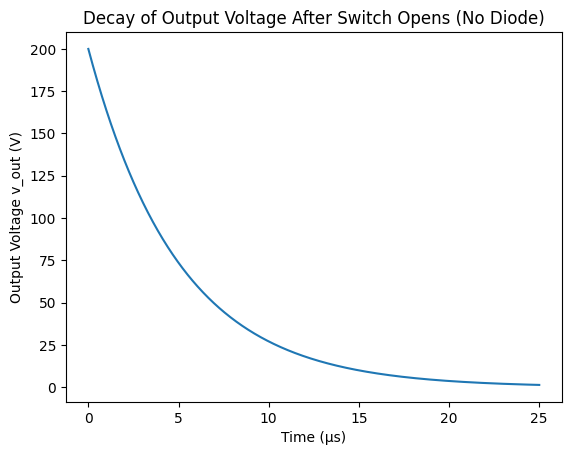
\includegraphics[width=0.6\textwidth]{plot.png}
    \end{center}
    
\end{answer}

\end{partquestion}

\end{mainquestion}
